\documentclass[12pt,letterpaper]{article}
\usepackage[latin1]{inputenc}
\usepackage{amsmath}
\usepackage{amsfonts}
\usepackage{amssymb}

% the above packages are the "base"

\usepackage{graphicx}

\usepackage{hyperref} % enable links within pdf
\hypersetup{colorlinks = true, linkcolor = black, urlcolor = blue}

 \usepackage[hang,flushmargin]{footmisc} % don't indent footnotes

\usepackage{ragged2e} % for justify{}
% Define a function to make a Ben-specific font :-)
 \newenvironment{ben}{\quote\justify\fontfamily{cmtt}\selectfont\small}{\par}

\setcounter{secnumdepth}{0}  % don't number sections (stars not needed)

% For making a multi-page box
\usepackage[most]{tcolorbox}

%%%%%%%%%%%%%%%%%%%%%%%%%%%%%%%%%

\author{}
\title{Structuring your project}
\date{}

\begin{document}

\maketitle
% \tableofcontents
% \pagebreak

 \begin{tcolorbox}[breakable, enhanced, before upper={\parindent15pt}]
 	\noindent
 	The following recommendations apply whether or not you plan to 
 	use version control software like \texttt{Git} to manage the contents of your project.
 	They apply equally if you plan to use \texttt{Dropbox} or the equivalent (which you should 
	\textit{most definitely} be using if you decide not to use version control).
\end{tcolorbox}

\section{Developing a project mindset} \label{projectmindset}

Like many grad students, I finished my thesis with
\begin{itemize}
	\item one main folder called \texttt{Data} with a bunch of sub-folders containing the various data sets (many in MS Excel format) and some relational databases (MS Access) that I'd collected or collated over the years;
	\item one main folder called \texttt{R} with sub-folders containing the R codes for each of my chapters, side projects, and undeveloped analysis beginnings;
	\item one main folder called \texttt{Mathematica} that similarly contained a bunch of sub-folders for various projects;
	\item one main folder called \texttt{Manuscripts} that contained all my writing and chapters that I'd attempted or completed;
\end{itemize}
and a bunch more similar folders all variously named and ``type-specific''.
Most of all these were within my overall \texttt{Research} folder.
You might currently have something similar for your thesis and any other research you're working on 
(Fig.~\ref{fig:old_figs}).

\begin{figure}[!h]
	\centering
	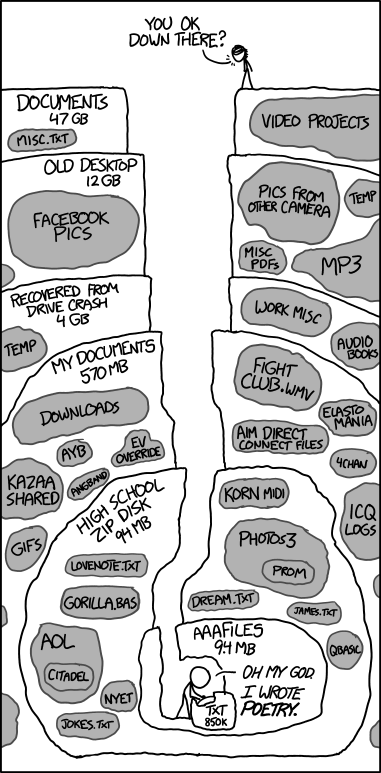
\includegraphics[width=0.5\linewidth]{figs/xkcd_old_files}
	\caption{Old files (source: \url{http://xkcd.com/1360/})}
	\label{fig:old_figs}
\end{figure}

Turns out that's a poor way to organize your work for a variety of reasons, including 
the ease of backing-up new data and code;
the easy of tracing errors in your data and code;
the ease of performing the seemingly simple act of reproducing (or just rerunning) past work
(by yourself or someone else);
and
the ease with which you might expand upon or modify (branch off) your prior work.

I now organize my work using a \emph{project mindset}.  
I don't do this for each and every nascent project idea or analysis I try out, 
but I do use it for ``definitely doing this'' projects 
(i.e.~planned-out ideas for a manuscript or for collaborative projects).
In a project mindset, 
(almost) everything associated with a given project is contained within one main, project-specific folder.

A project mindset encourages \emph{deliverables-based} thinking. 
By identifying and naming the "definitely doing this" projects, 
I am encouraged to consider the project's own project-specific priorities. 
For example, for each project I am forced to think clearly about what the project is fundamentally about by having to name the folder. 
Asking "what should this project folder be called?" 
(and insisting on an \emph{informative name}!)
is pretty close to asking "what is this project about?"
\unskip
\footnote{Folder and file naming conventions are something we'll come back to when we talk about Coding Best Practices.} 
		
A project mindset promotes better time management. 
For instance, all my project folders are contained within three superfolders: 
Active, Complete and Archive. 
The Active folder contains stuff I am working on right now.
The folders within Complete are renamed with the year as a prefix for ease of finding. 
Archive is for stuff that is on the back-burner. 
In this setup, 
the folders within the Active folder 
-- each with a name that reminds me of the objective for that project -- 
becomes a kind of high-level To-Do list. 
The motivational goal is to be able drag those folders from Active to Complete. 
Crucially, if the Active folder gets too full, 
I know I will not be able to succeed in moving project folders because my attention has become too divided. 
So then I ask myself which are the most important few projects to me, 
and drag the rest to the Archive folder. 
It's not that I can't do them later. 
Rather, it's just recognizing that 
(a) they are not done yet, and 
(b) they are not the first, second or even third priority. 
If both (a) and (b) are true, into the Archive folder they go!

Finally, a project mindset is key to the effective use of version control software like \texttt{Git}.
	
All that said, defining ``a project'' can get difficult 
(esp.~within your thesis work), 
so a fair bit of thought is typically needed.
It's not trivial, but does become quicker with time (and seeing what others do).


\section{Structuring your Project folder} \label{projectfolder}

What does a project mindset look like in practice?
Well, for most projects, within each project folder, 
I start off by creating the following sub-folders:

\begin{tabular}{ll}
 \texttt{data} & the data required for the project \\
 \texttt{code} & all the scripts needed to perform the analyses \\
 \texttt{results} & all the output of the analyses \\
 \texttt{figs} & final figures that go into the manuscript\\
 \texttt{tables} & final tables that go into the manuscript\\
 \texttt{manuscript} & manuscript derived from the project\\
\end{tabular}

\noindent
The first three 
--- \texttt{data}, \texttt{code} and \texttt{results} (or \texttt{output}) ---
are definites for any project.
The \texttt{data} folder contains \texttt{original} and \texttt{cleaned} or otherwise derived data in subfolders.
\unskip
\footnote{Leaving your original data as untouched as possible is something we'll come back to during Coding Best Practices.} 
Within \texttt{code} I might have \texttt{R} and/or \texttt{Mathematica} subfolders, as relevant.
I use \texttt{figs}, \texttt{tables}, and \texttt{manuscript} for projects that will form the basis of a manuscript
(almost every project at this point).
The contents of \texttt{figs} and \texttt{tables} differs from the interim, exploratory, or otherwise rough-and-dirty figures and tables that go into the \texttt{results} folder.


\section{Project folders and \texttt{Git} repositories}

When using version control software you'll typically have just one \emph{repository} associated with each one of your projects.  
A \emph{project folder} is thus synonymous with a \emph{repository}.  
As a result of using version control software you'll also have a few additional files in your project folder.
That is, each project folder should have a \texttt{README.md} file; 
a text file written in \texttt{Markdown} that describes the project and the folder's contents.
(We'll come back to writing with \texttt{Markdown} later in the course.)
\unskip
\footnote{In fact, it's very good practice to have a \texttt{README.md} file in each of the ``important'' subfolders of your project, too, each identifically named (so that \texttt{GitHub} will display it when looking in the folder through a browser) and describing what's in the subfolder.}
If you're using \texttt{R-Studio}, 
then you may also have an \texttt{.Rproj} file in which \texttt{RStudio} saves your project-specific settings and preferences.  
Your project folder will also have several \texttt{Git} files in it that, 
by the default settings of your operating system, 
will remain hidden unless you want them to be shown.
These include a \texttt{.gitignore} file
(which we'll discuss when we talk about \texttt{Git}.)


\subsection{Keeping some things private}

There are many reasons to make your research products
---which include your data and code---
publicly accessible.
Having a project mindset and using \texttt{Git} makes it very easy to do that.
All you have to do is make your \texttt{Git} repository public on \texttt{GitHub},
either when creating the repository or by changing a private repository's setting to public.
\unskip
\footnote{Ideally you'll also place these products in a permanent repository, like \texttt{FigShare}, \texttt{Data Dryad}, etc.).}
But you probably don't want to showcase all the trials and tribulations of your manuscript writing
(which likely include records of the baseless bashings of Reviewer \#2)).
You may also be in a situation where you don't have the requisite permissions to make all or some of your data public.
Or your data may entail files that are so large that they make using \texttt{Git} and \texttt{GitHub} impracticle or not possible.
In such situations you may not want to include your \texttt{manuscript} or your \texttt{data} subfolders in the same folder (repository) as the rest of the project.

There are a number of possible solutions:
\unskip
\footnote{These will likely make more sense after we've talked about using \texttt{Git} 
and about the difference between specifying \emph{full} versus \emph{relational} paths
(which we'll discuss in Coding Best Practices).}

\begin{enumerate}
\item Create an additional project folder specific to your data or manuscript.  
Place it either in \texttt{Dropbox} (if necessary) or make it its own repository to get the benefits of using \texttt{Git}.  
This option requires specifying the \emph{full} path between repositories to access data/files from one in the other. 
\item  Go ahead and create the subfolder in your main project folder and, 
before ever committing it, 
add the name of that subfolder to the repository's \texttt{.gitignore} file.
This option will keep all your project files together, allow you to use \emph{relational} paths within it, 
but loses the benefits of version control for the contents of the subfolder. 

\item  Combine and get the best of options (1) and (2) by
\begin{enumerate}
	\item adding the subfolder to your project repository,
	\item adding that subfolder to \texttt{.gitignore},
	\item creating an empty text file in that folder (so that \texttt{Git} sees the folder),
	\item creating another subfolder within the first,
	\item creating and cloning a second (private) repository into the subfolder.
\end{enumerate}
\end{enumerate}

\noindent
With option (3) you have two repositories to manage, \texttt{Git} doesn't "see" the "sub-repository" inside the main project folder, and you get all the benefits of the projects mindset and of using version control. 


\subsection{Using \texttt{Git} with \texttt{Dropbox} or \texttt{GoogleDrive}}

I do still use a combination of \texttt{Git} and \texttt{Dropbox} for some projects based on my needs
or those of my collaborators, 
but to the extent that it is possible it is better to organize things within a single project-specific folder.
Note, however, that you're asking for trouble if you put a \texttt{Git} repository within a \texttt{Dropbox} or \texttt{GoogleDrive} folder, or vice versa.  
Don't do it!  
If you really, realy want or need to 
(e.g., if your collaborator doesn't want to learn Git but does want to use Dropbox), 
then see \url{https://github.com/anishathalye/git-remote-dropbox}.

\end{document}
